\documentclass[    
  12pt, 
  compress,
  aspectratio=169,
  %handout, 
  blue
  ]{beamer}

%-----------------------------------------------------
% PACKAGES USADOS
%-----------------------------------------------------  
\usepackage{beamerthemesplit} 
\usecolortheme{sidebartab}
\usetheme[secheader]{Boadilla}
\usepackage{graphicx}
\graphicspath{ {assets} }
\setbeamertemplate{headline}{\hfill
\includegraphics[width=1.1cm]{tche}\hspace{0.2cm}\vspace{-0.8cm}}

%-------------------------------------------------------
%INFOS
%-------------------------------------------------------
\title{Migração de Carreira-Você também pode!}    
\author[Talita Silveira]{Talita Silveira\\[2ex] 
\includegraphics[scale=0.25]{logo}}               
\institute{Invillia | PagSeguro}      
\date{\today}    

%-------------------------------------------------------
%INICIO DO COCUMENTO
%-------------------------------------------------------
\begin{document}

%-------------------------------------------------------
%PRIMEIRO SLIDE
%-------------------------------------------------------
\begin{frame}
\titlepage
\usebeamerfont{institute} contato: \url{silveira.tacristina@gmail.com}
\end{frame}
\note{Talk for 30 minutes} 
\section[Migração de carreira]{}
\section{Você também pode!}

%-------------------------------------------------------
%SEGUNDO SLIDE
%-------------------------------------------------------

\begin{frame}
\frametitle{ Um pouco sobre mim!}   
\begin{columns}[c]
\column{0.5\textwidth}  
\begin{itemize}
\item<1-> Formação 
\item<2-> Trabalho  
\item<3-> Carreira
\item<4-> Linux
\end{itemize}
\column{0.5\textwidth}
\centering
\begin{figure}

\includegraphics[scale=0.1]{eu}
\end{figure}
\end{columns}
\end{frame}

%-------------------------------------------------------
%TERCEIRO SLIDE
%-------------------------------------------------------

\begin{frame}
\frametitle{ Migrando de área}   
\begin{columns}[c]
\column{0.5\textwidth}
\begin{itemize}
\item<1-> Motivação 
\end{itemize}
\begin{block}{Trecho da matéria}
“A administradora de empresas Isabel Nasser, cofundadora da startup de automatização de operações de comércio exterior Kestraa,  de São Paulo, ficou chocada quando um estagiário em desenvolvimento de softwares que estava terminando a faculdade recusou um salário de 12.000 reais com carteira assinada e generosos benefícios para ser efetivado.”
\end{block}
\column{0.5\textwidth}
\centering
\begin{figure}
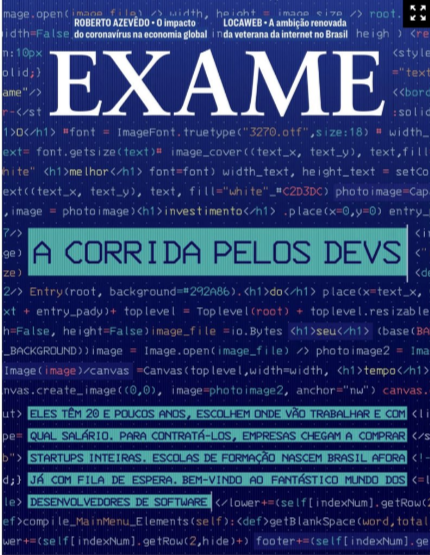
\includegraphics[scale=0.3]{revista}
\end{figure}
\end{columns}
\end{frame}

%-------------------------------------------------------
%QUINTO SLIDE
%-------------------------------------------------------
\begin{frame}
\frametitle{ Requisitos}   

\begin{itemize}
\item<1-> Soft Skills
\item<2-> Hard Skills  
\item<3-> Conhecimento em idiomas
\item<4-> Qual o perfil procurado por times reais?
\end{itemize}

\end{frame}

%-------------------------------------------------------
%SEXTO SLIDE
%-------------------------------------------------------
\begin{frame}
\frametitle{ Soft Siklls}   

\begin{itemize}
\item<1-> Comunicação
\item<2-> Flexibilidade
\item<3-> Gerenciamento de tempo
\item<4-> Liderança
\item<5-> Motivação
\item<6-> Persuasão
\item<6-> Trabalho em equipe
\item<6-> Inteligência emocional
\end{itemize}

\end{frame}
%-------------------------------------------------------
%SETIMO SLIDE
%-------------------------------------------------------
\begin{frame}
\frametitle{ Hard Siklls}   

\begin{itemize}
\item<1-> Proficiência em inglês
\item<2-> Domínio de Java
\item<3-> Metodologias de desenvolvimento de software
\item<4-> Domínio de git
\item<5-> Domínio de Javascript
\item<6-> Domínio de CSS
\end{itemize}

\end{frame}

%-------------------------------------------------------
%OITAVO SLIDE
%-------------------------------------------------------
\begin{frame}
\frametitle{ Idiomas e Perfil}   
\begin{columns}[c]
\column{0.5\textwidth}  
\begin{itemize}
\item<1-> Conhecimento em Inglês 
\item<2-> Qual o perfil procurado por times reais?  
\end{itemize}
\column{0.5\textwidth}
\centering
\begin{figure}
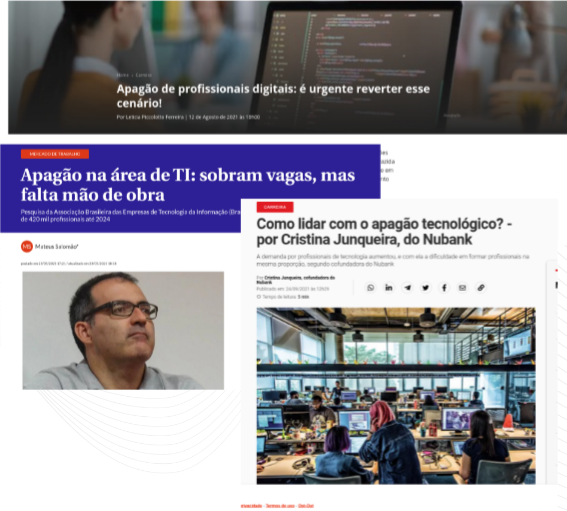
\includegraphics[scale=0.4]{apagao}
\end{figure}
\end{columns}
\end{frame}

%-------------------------------------------------------
%NONO SLIDE
%-------------------------------------------------------
\begin{frame}
\frametitle{ Linux - Porque Linux?}   
\begin{columns}[c]
\column{0.5\textwidth}  
\begin{itemize}
\item<1-> Porque usar Linux?
\item<2-> Como se tornar um usuário linux
\item<3-> O bash e shell script e sua importância
\end{itemize}
\column{0.5\textwidth}
\centering
\begin{figure}

\includegraphics[scale=0.3]{programas}
\end{figure}
\end{columns}
\end{frame}
%-------------------------------------------------------
%DÉCIMO SLIDE
%-------------------------------------------------------
\begin{frame}
\frametitle{ Outros conhecimentos}   
\begin{columns}[c]
\column{0.5\textwidth}  
\begin{itemize}
\item<1-> Estrutura de dados
\item<2-> Git
\item<3-> Redes/ sistemas distribuídos
\item<4-> Hardware do seu computador
\end{itemize}
\column{0.5\textwidth}
\centering
\begin{figure}

\includegraphics[scale=0.3]{estrutura}
\end{figure}
\end{columns}
\end{frame}
%-------------------------------------------------------
%11- SLIDE
%-------------------------------------------------------
\begin{frame}
\frametitle{ Dicas}   

\begin{itemize}
\item<1-> Documentação como primeira orientação para o desenvolvimento do aprendizado
\item<2-> Conhecimento sobre hardware e sistemas operacionais -daí o motivo de entender melhor o funcionamento linux
\item<3-> Curiosidade sobre novas tecnologias e disposição em aprender

\end{itemize}

\end{frame}
%-------------------------------------------------------
%12- SLIDE
%-------------------------------------------------------
\begin{frame}
\frametitle{ Materiais bacanas!}   

\begin{itemize}
\item<1-> https://loiane.training/
\item<2->https://www.youtube.com/c/loianegroner
\item<3->https://www.youtube.com/user/linuxtipscanal
\item<4->https://blog.4linux.com.br/
\item<5->https://www.vivaolinux.com.br/
\item<6->https://www.youtube.com/c/progshelllinux/videos
\item<7->https://www.youtube.com/c/FabioAkita1990
\item<8->https://www.youtube.com/c/TerminalRootTV/videos


\end{itemize}

\end{frame}
%-------------------------------------------------------
%13- SLIDE
%-------------------------------------------------------
\begin{frame}
\frametitle{ Para além do tecnico - Livros}   
\begin{columns}[c]
\column{0.5\textwidth}  
\begin{itemize}
\item<1-> Mais espero que o diabo - Napoleon Hill.
\end{itemize}
\column{0.5\textwidth}
\centering
\begin{figure}
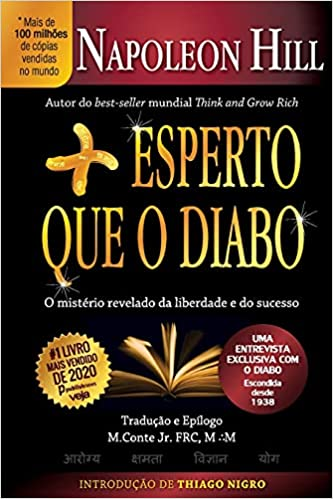
\includegraphics[scale=0.3]{diabo}
\end{figure}
\end{columns}
\end{frame}

%-------------------------------------------------------
%14- SLIDE
%-------------------------------------------------------
\begin{frame}
\frametitle{ Para além do tecnico - Livros}   
\begin{columns}[c]
\column{0.5\textwidth}  
\begin{itemize}
\item<1-> Comunicação não violenta - Marshall B. Rosenberg.
\end{itemize}
\column{0.5\textwidth}
\centering
\begin{figure}

\includegraphics[scale=0.3]{comunicacao}
\end{figure}
\end{columns}
\end{frame}

%-------------------------------------------------------
%15- SLIDE
%-------------------------------------------------------
\begin{frame}
\frametitle{ Para além do tecnico - Livros}   
\begin{columns}[c]
\column{0.5\textwidth}  
\begin{itemize}
\item<1-> Inteligencia Emocional - Daniel Goleman.
\end{itemize}
\column{0.5\textwidth}
\centering
\begin{figure}
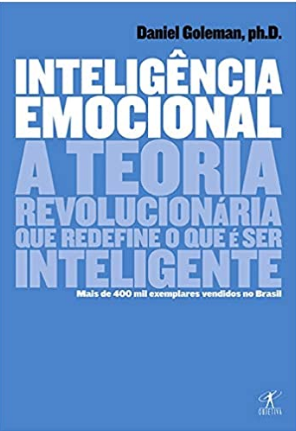
\includegraphics[scale=0.5]{inteligencia}
\end{figure}
\end{columns}
\end{frame}

%-------------------------------------------------------
%16- SLIDE
%-------------------------------------------------------
\begin{frame}
\frametitle{ Metodologias}   
\begin{columns}[c]
\column{0.5\textwidth}  
\begin{itemize}
\item<1-> Aprenda sobre metodologias.
\end{itemize}

\begin{columns}[c]
\column{0.5\textwidth} 
\centering
\begin{figure}
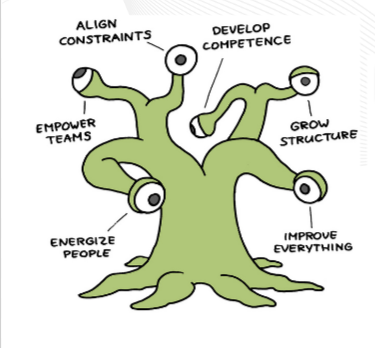
\includegraphics[scale=0.3]{metodoloia1}
\end{figure}

\column{0.5\textwidth}
\begin{figure}
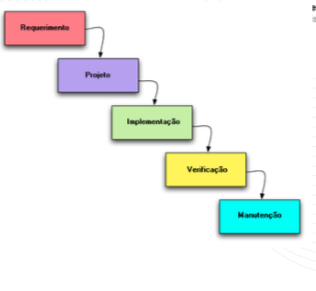
\includegraphics[scale=0.3]{metodologia2}
\end{figure}

\end{columns}

\column{0.5\textwidth}
\centering
\begin{figure}
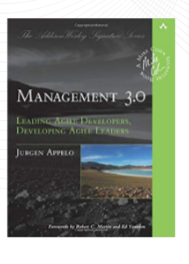
\includegraphics[scale=0.3]{metodoloia3}
\end{figure}
\end{columns}
\end{frame}
\end{document}